\documentclass{article}
\usepackage{import}
\usepackage[ruled]{algorithm2e}
\usepackage[shortlabels]{enumitem}
\usepackage{hyperref}
\usepackage{subcaption}
\hypersetup{
    colorlinks=true,
    linkcolor=blue,
    filecolor=magenta,      
    urlcolor=cyan,
    pdftitle={Overleaf Example},
    pdfpagemode=FullScreen,
    }
\subimport*{./}{macro}

\setlength\parindent{0px}

\begin{document}
\setcounter{aprob}{0}
\title{Homework \#2}
\author{
    \normalsize{CSE 446/546: Machine Learning}\\
    \normalsize{Prof. Kevin Jamieson}\\
    \normalsize{Due: November 6, 2023 11:59pm}\\
    \normalsize{Points A: 104; B: 20}
}
\date{{}}
\maketitle
\begin{sloppypar}
% \noindent Please review all homework guidance posted on the website before submitting it to Gradescope. Reminders:
% \begin{itemize}
%     \item Make sure to read the ``What to Submit'' section following each question and include all items.
%     \item Please provide succinct answers and supporting reasoning for each question. Similarly, when discussing experimental results, concisely create tables and/or figures when appropriate to organize the experimental results. All explanations, tables, and figures for any particular part of a question must be grouped together.
%     \item For every problem involving generating plots, please include the plots as part of your PDF submission.
%     \item When submitting to Gradescope, please link each question from the homework in Gradescope to the location of its answer in your homework PDF. Failure to do so may result in deductions of up to 10\% of the value of each question not properly linked. For instructions, see \url{https://www.gradescope.com/get_started#student-submission}.
%     \item If you collaborate on this homework with others, you must indicate who you worked with on your homework by providing a complete list of collaborators on the first page of your assignment. Make sure to include the name of each collaborator, and on which problem(s) you collaborated. Failure to do so may result in accusations of plagiarism. You can review the course collaboration policy at \url{https://courses.cs.washington.edu/courses/cse446/23au/assignments/}
%     \item For every problem involving code, please include all code you have written for the problem as part of your PDF submission \emph{in addition to} submitting your code to the separate assignment on Gradescope created for code. Not submitting all code files will lead to a deduction of up to 10\% of the value of each question missing code.  
% \end{itemize}

% Not adhering to these reminders may result in point deductions. \\

\clearpage{}

\section*{Conceptual Questions}

\begin{aprob}
    The answers to these questions should be answerable without referring to external materials.
    Briefly justify your answers with a few words.
    \begin{enumerate}
      \item \points{2} Explain why a L1 norm penalty is more likely to result in sparsity (a larger number of 0s) in the weight vector, as compared to the L2 norm.
      \item \points{2} In at most one sentence each, state one possible upside and one possible downside of using the following regularizer: $\left(\sum_{i}\left|w_{i}\right|^{0.5}\right)$.
      \item \points{2} True or False: If the step-size for gradient descent is too large, it may not converge.
      \item \points{2} In at most one sentence each, state one possible advantage of SGD over GD (gradient descent), and one possible disadvantage of SGD relative to GD.
      \item \points{2} Why is it necessary to apply the gradient descent algorithm on logistic regression but not linear regression?
    \end{enumerate}
    
    \subsection*{What to Submit:}
    \begin{itemize}
        \item \textbf{Part c:} True or False. 
        \item \textbf{Parts a-e:} Brief (2-3 sentence) explanation.
    \end{itemize}
    
    \subsection*{Answers}
    \begin{enumerate}
        \item Since L1 norm penalty leads to many coefficient to become zeros. 
        While L2 norm penalty with small but non-zero coefficient.
        \item Upsie: provide zero sparsity like L1 norm. Downside: this regularizer changes faster and faster when close to zero, may complicate garadient computation.
        \item True. The algorithm may overshot the optimal solution if the step-size is too large. It may bounce back and forth across the minimal solution.
        \item SGD converge faster than GD. Randomness in SGD may have issue like inconsistent result.
        \item Logistic regression is non-linear non-convex function thus does not have a closed form. It needs GD to iterate find optimal sulution.
    \end{enumerate}
\end{aprob}

\newpage

\section*{Convexity and Norms}

\begin{aprob}
    A \emph{norm} $\|\cdot\|$ over $\R^n$ is defined by the properties:
    (\textit{i}) non-negativity: $\|x\|\geq 0$ for all $x \in \R^n$ with equality if and only if $x=0$,
    (\textit{ii}) absolute scalability: $\|a \, x\| = |a| \, \|x\|$ for all $a \in \R$ and $x \in \R^n$, 
    (\textit{iii}) triangle inequality: $\|x+y\| \leq \|x\| + \|y\|$ for all $x,y \in \R^n$.
    \begin{enumerate}
      \item \points{3} Show that $f(x) = \left( \sum_{i=1}^n |x_i| \right)$ is a norm. (Hint: for (\textit{iii}), begin by showing that $|a+b|\leq |a| + |b|$ for all $a,b \in \R$.)
      \item \points{2} Show that $g(x) = \left(\sum_{i=1}^n |x_i|^{1/2}\right)^2$ is not a norm. (Hint: it suffices to find two points in $n=2$ dimensions such that the triangle inequality does not hold.)
    \end{enumerate} 
    Context: norms are often used in regularization to encourage specific behaviors of solutions. If we define  $\| x \|_p := \left( \sum_{i=1}^n |x_i|^{p} \right)^{1/p}$ then one can show that $\| x \|_p$ is a norm for all $p \geq 1$. 
    The important cases of $p=2$ and $p=1$ correspond to the penalty for ridge regression and the lasso, respectively. 
    
    \subsection*{What to Submit:}
    \begin{itemize}
        \item \textbf{Parts a, b:} Proof.
    \end{itemize}

    \subsection*{Answers}
    \begin{enumerate}
        \item $f(x)=\sum_{i=1}^{n} |x_i| = |x_1|+|x_2|+\dots+|x_n|$. Since each term is a non negative value, we conclude that $f(x)\ge 0$.
        \begin{align*}
            f(ax) &=\sum_{i=1}^{n} |ax_i| \\
            &= |ax_1|+|ax_2|+\dots+|ax_n| \\
            &= a|x_1|+a|x_2|+\dots+a|x_n|\\
            &=a(|x_1|+a|x_2|+\dots+a|x_n|)\\
            &=af(x)
        \end{align*}
        \item We'll try to prove by finding a counterexample. First, let $n=2$, 
        assume we have two positive vector $x$, $y$.
        \begin{align*}
            g(x) &= (\sum_{i=1}^n |x_i|^{1/2})^2 \\
            &= (\sqrt{|x_1|}+\sqrt{|x_2|})^2 \\
            &= x_1 + x_2 + 2\sqrt{x_1 x_2}
        \end{align*}
        Similarly, $g(y) =  y_1 + y_2 + 2\sqrt{y_1 y_2}$
        \begin{align*}
            g(x) + g(y) &= x_1 + x_2 + 2\sqrt{x_1 x_2} + y_1 + y_2 + 2\sqrt{y_1 y_2} \\
            &= (x_1+y_1) + (x_2+y_2) + 2(\sqrt{x_1 x_2} + \sqrt{y_1 y_2})
        \end{align*}
        \begin{align*}
            g(x + y) &= (\sum_{i=1}^n |x_i+y_i|^{1/2})^2 \\
            &= (x_1+y_1) + (x_2+y_2) + 2\sqrt{(x_1+y_1) (x_2+y_2)} \\
            &= (x_1+y_1) + (x_2+y_2) + 2\sqrt{x_1 x_2 + y_1 y_2 + x_1 y_2 + x_2 y_1}
        \end{align*}
        If $g(x)$ is a norm, the triangle inequality should hold.
        \begin{align*}
            g(x) +g(y) &\ge g(x+y) \\
            (x_1+y_1) + (x_2+y_2) + 2(\sqrt{x_1 x_2} + \sqrt{y_1 y_2}) &\ge (x_1+y_1) + (x_2+y_2) + 2\sqrt{x_1 x_2 + y_1 y_2 + x_1 y_2 + x_2 y_1} \\
            \sqrt{x_1 x_2} + \sqrt{y_1 y_2} &\ge \sqrt{x_1 x_2 + y_1 y_2 + x_1 y_2 + x_2 y_1} \\
            x_1 x_2 + y_1 y_2 + 2\sqrt{x_1 x_2 y_1 y_2} &\ge x_1 x_2 + y_1 y_2 + x_1 y_2 + x_2 y_1 \\
            2\sqrt{x_1 x_2 y_1 y_2} &\ge x_1 y_2 + x_2 y_1 \\
            0 &\ge  x_1 y_2 + x_2 y_1 - 2\sqrt{x_1 x_2 y_1 y_2} \\
            0 & \ge (\sqrt{x_1 y_2} + \sqrt{x_2 y_1})^2
        \end{align*}
        However, $(\sqrt{x_1 y_2} + \sqrt{x_2 y_1})^2 > 0$ is always true. 
        This violates the trianglar inequality. So that $g(x)$ is not a norm.
    \end{enumerate}
\end{aprob}


\begin{aprob}
    \points{2} A set $A \subseteq \R^n$ is \emph{convex} if $\lambda x + (1-\lambda) y \in A$ for all $x,y\in A$ and $\lambda \in [0,1]$.
    For each of the grey-shaded sets below (I-II), state whether each one is convex, or state why it is not convex using any of the points $a,b,c,d$ in your answer. 
    
    \begin{figure}[!h]
        \centering
        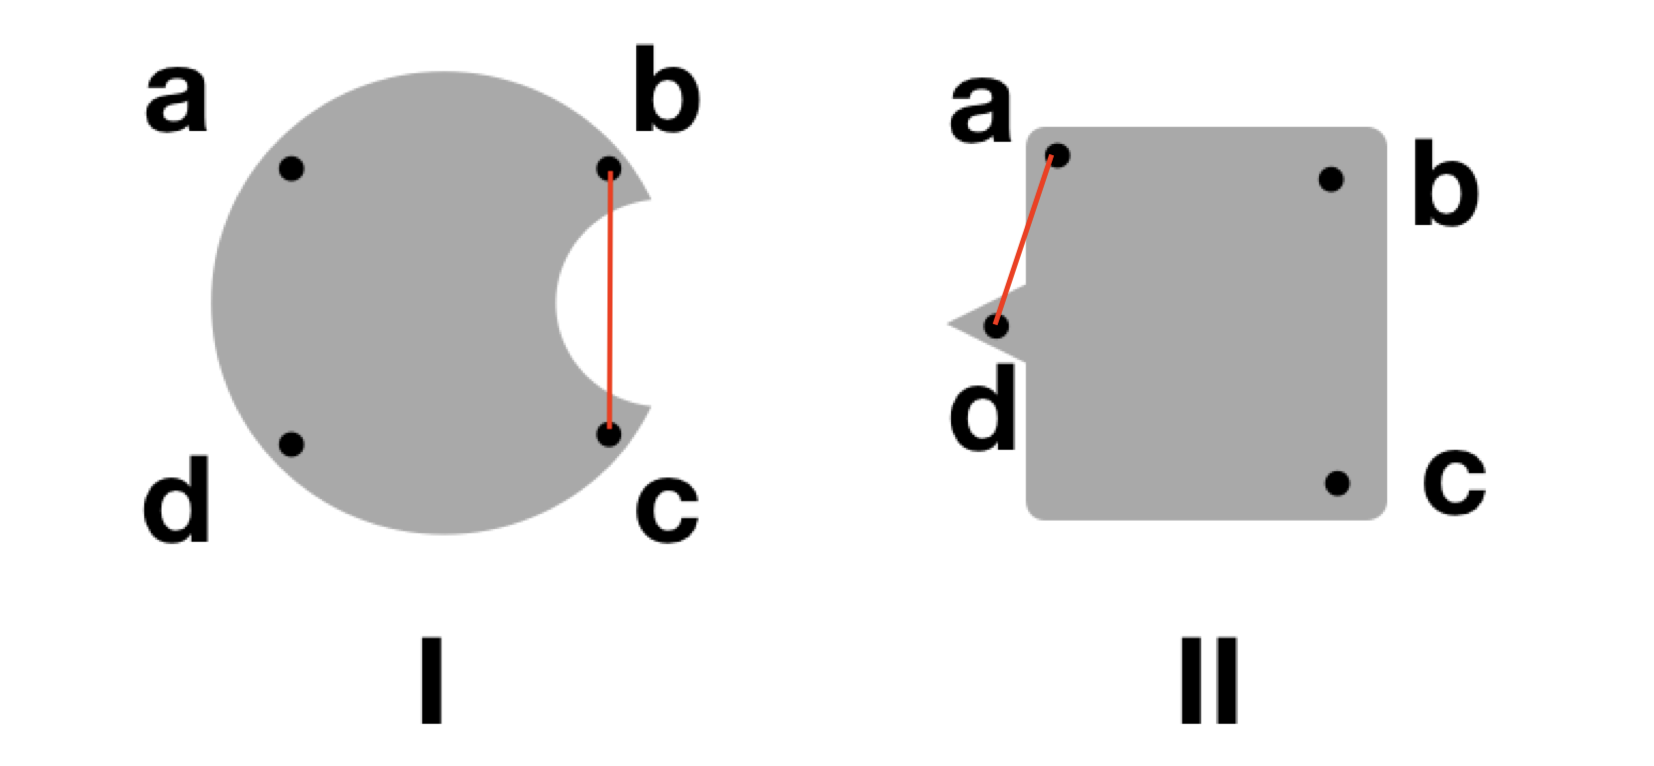
\includegraphics[width=.6\textwidth]{./img/convex_shapes2.png}
        \caption{Convex Shapes}
        \label{fig:conve_shapes}
    \end{figure}

    \subsection*{What to Submit:}
    \begin{itemize}
        \item \textbf{Parts I, II:} 1-2 sentence explanation of why the set is convex or not.
    \end{itemize}
    \subsection*{Answers}
    \begin{itemize}
        \item Both set \textbf{I, II} are not convex.
        For set \textbf{I}, part of the line between point $b$ and $c$ lies outside of the set.
        While for set \text{II}, draw a line between point $a$ and $d$, we can see not all points on the line are within the domain of the set.
        See figure \ref{fig:conve_shapes}
    \end{itemize}
\end{aprob}

\begin{aprob}
    \points{2} We say a function $f: \R^d \rightarrow \R$ is convex on a set $A$ if $f(\lambda x + (1-\lambda) y) \leq \lambda f(x) + (1-\lambda) f(y)$ for all $x,y\in A$ and $\lambda \in [0,1]$. For each of the functions shown below (I-II), state whether each is convex on the specified interval, or state why not with a counterexample using any of the points $a,b,c,d$ in your answer.

    \begin{enumerate}
        \item Function in panel I on $[a,c]$
        \item Function in panel II on $[a,d]$
    \end{enumerate}
    
    \begin{figure}[!h]
        \centering
        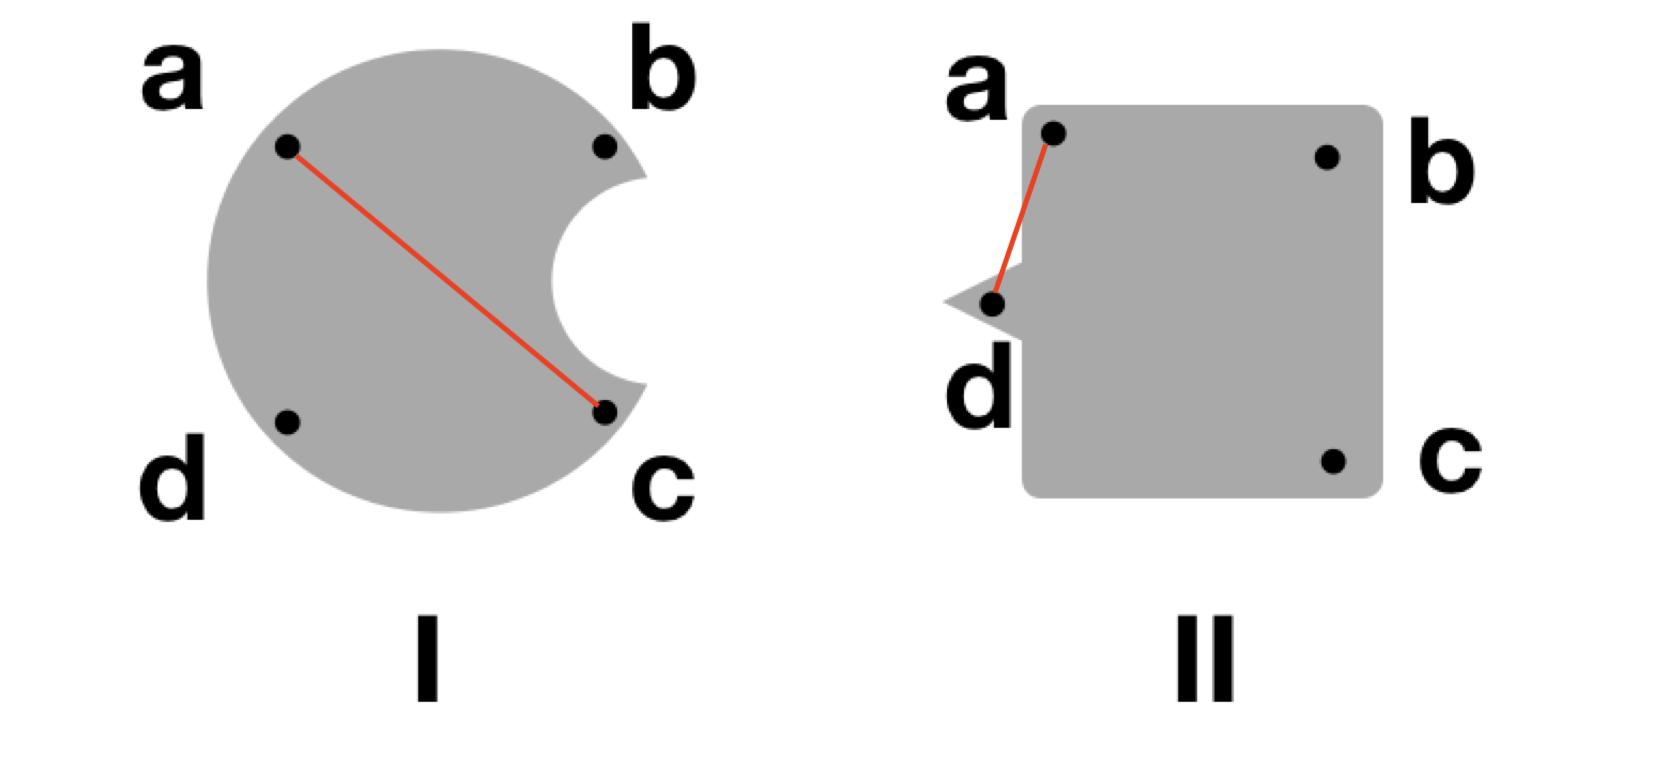
\includegraphics[width=.75\textwidth]{./img/convex_functions2.png}
        \caption{Convex Functions}
        \label{fig:convex_functions}
    \end{figure}

    \subsection*{What to Submit:}
    \begin{itemize}
        \item \textbf{Parts a, b:} 1-2 sentence explanation of why the function is convex or not.
    \end{itemize}
    \subsection*{Answers}
    \begin{itemize}
        \item In panel I on $[a, c]$, the line segment lies within the set (Figure \ref{fig:convex_functions}). 
        Which means $\lambda x + (1-\lambda) y$ in the set, so that $f$ is convex in set I.
        \item In panel II on $[a, d]$, we find part of the line segment lies outside of the set ((Figure \ref{fig:convex_functions}). 
        We can find points that let $\lambda x + (1-\lambda) y$ not in the set, so $f$ is not convex in this set.
    \end{itemize}
\end{aprob}

\newpage

% \section*{Lasso on a Real Dataset}
% Given $\lambda >0$ and data $\Big (x_i,y_i \Big)_{i=1}^n$, the Lasso is the problem of solving
% \begin{equation*}\label{eq:lasso}
%   \arg\min_{{w}\in \R^d, b \in \R} \sum_{i=1}^n { (x_i^T {w} + b - {y}_i)^2 }
%     + \lambda \sum_{j=1}^d |{w}_j| 
% \end{equation*}
% where $\lambda$ is a regularization parameter.
% For the programming part of this homework, you will implement the iterative shrinkage thresholding algorithm shown in Algorithm~\ref{alg:ista} to solve the Lasso problem in \texttt{ISTA.py}. This is a variant of the subgradient descent method and a more detailed discussion can be found in these \href{https://www.stat.cmu.edu/~ryantibs/convexopt-F15/lectures/08-prox-grad.pdf}{slides}. You may use common computing packages (such as \texttt{numpy} or \texttt{scipy}), but do not use an existing Lasso solver (e.g., of \texttt{scikit-learn}).

% \begin{algorithm}[h]
%     \caption{Iterative Shrinkage Thresholding Algorithm for Lasso}
%     \label{alg:ista}
%     \KwIn{Step size $\eta$}
%     \While{not converged}{
%     $b'\leftarrow b-2\eta\sum_{i=1}^n(x_i^Tw+b-y_i)$\\
%       \For{$k \in \{1,2,\cdots d\}$} {
%         $w'_k\leftarrow w_k-2\eta\sum_{i=1}^nx_{i,k}(x_i^Tw+b-y_i)$\\
%         $w'_k \leftarrow 
%         \left\{
%         \begin{array}{ll}
%           w'_k+2\eta\lambda  & w'_k < -2\eta\lambda\\
%           0 & w'_k\in [-2\eta\lambda, 2\eta\lambda]\\
%           w'_k-2\eta\lambda  & w'_k > 2\eta\lambda\\
%         \end{array}  
%         \right.
%         $\\
%       }
%       $b\leftarrow b'$, $w\leftarrow w'$\\
%     }
% \end{algorithm}

% Before you get started, the following hints may be useful:
% \begin{itemize}
%   \item Wherever possible, use matrix libraries for matrix operations (not \texttt{for} loops). This especially applies to computing the updates for $w$. While we wrote the algorithm above with a \texttt{for} loop for clarity, you should be able to replace this loop using equivalent matrix/vector operations in your code (e.g., \texttt{numpy} functions).
%   \item As a sanity check, ensure the objective value is nonincreasing with each step. 
%   \item It is up to you to decide on a suitable stopping condition.  A common criteria is to stop when no element of
%       ${w}$ changes by more than some small $\delta$ during an iteration.  If you need your algorithm to run faster,
%       an easy place to start is to loosen this condition.
%   \item You will need to solve the Lasso on the same dataset for many values of $\lambda$.  This
%       is called a regularization path.  One way to do this efficiently is to start at a large $\lambda$, and then for each consecutive solution, initialize the algorithm with the previous solution, decreasing $\lambda$ by a constant ratio (e.g., by a factor of $2$).
%   \item The smallest value of $\lambda$ for which the solution $\widehat{w}$ is entirely zero is given by
%        \begin{align}
%            \lambda_{max} = \max_{k=1,\dots,d} 2 \left|\sum_{i=1}^n {x}_{i,k} \left({y}_i - \left(\frac{1}{n} \sum_{j=1}^n y_j \right)\right)\right|
%            \label{eqn:lasso-lambdamax}
%        \end{align}
%       This is helpful for choosing the first $\lambda$ in a regularization path. 
% \end{itemize}

\begin{aprob}
    We will first try out your solver with some synthetic data.
    A benefit of the Lasso is that if we believe many features are irrelevant for predicting ${y}$, the Lasso can be used to enforce a sparse solution, effectively differentiating between the relevant and irrelevant features.
    Suppose that ${x} \in \mathbb{R}^d, y \in \mathbb{R}, k < d$, and data are generated independently according to the model $y_i = w^T x_i + \epsilon_i$ where
    \begin{align}
        w_j = \begin{cases} j/k & \text{if } j \in \{1,\dots,k\} \\
        0 & \text{otherwise}
        \end{cases}\label{eqn:lasso-model}
    \end{align} 
    and $\epsilon_i \sim \mathcal{N}(0, \sigma^2)$ is noise (note that in the model above $b=0$). We can see from Equation \eqref{eqn:lasso-model} that since $k < d$ and $w_j = 0$ for $j > k$, the features $k + 1$ through $d$ are irrelevant for predicting $y$.
    
    Generate a dataset using this model with $n = 500, d = 1000, k = 100,$ and $\sigma = 1$. You should generate the dataset such that each $\epsilon_i \sim \mathcal{N}(0, 1)$ , and $y_i$ is generated as specified above. You are free to choose a distribution from which the $x$'s are drawn, but make sure standardize the $x$'s before running your experiments.

    \begin{enumerate}
        \item \points{10} With your synthetic data, solve multiple Lasso problems on a regularization path, starting at $\lambda_{max}$ where no features are selected (see Equation \eqref{eqn:lasso-lambdamax}) and decreasing $\lambda$ by a constant ratio (e.g., 2) until nearly all the features are chosen. 
        In plot 1, plot the number of non-zeros as a function of $\lambda$ on the x-axis (Tip: use \verb|plt.xscale('log')|).
        \item \points{10} For each value of $\lambda$ tried, record values for false discovery rate (FDR) (number of incorrect nonzeros in $\widehat{w}$/total number of nonzeros in $\widehat{w}$) and true positive rate (TPR)
        (number of correct nonzeros in $\widehat{w}$/k). Note: for each $j$, $\widehat{w}_j$ is an incorrect nonzero if and only if $\widehat{w}_j \neq 0$ while $w_j = 0$.
        In plot 2, plot these values with the x-axis as FDR, and the y-axis as TPR.
          
        Note that in an ideal situation we would have an (FDR,TPR) pair in the upper left corner. We can always trivially achieve $(0,0)$ and $(\tfrac{d-k}{d},1)$.
          
        \item \points{5} Comment on the effect of $\lambda$ in these two plots in 1-2 sentences.
  \end{enumerate}
  
  \subsection*{What to Submit:}
    \begin{itemize}
        \item \textbf{Part a:} Plot 1.
        \item \textbf{Part b:} Plot 2.
        \item \textbf{Part c:} 1-2 sentence explanation.
        \item \textbf{Code} on Gradescope through coding submission
        \item \textbf{All code you wrote} in the write-up, with correct page mapping.
    \end{itemize}
    \begin{figure}[!h]
        \begin{subfigure}{.45\textwidth}
            \centering
            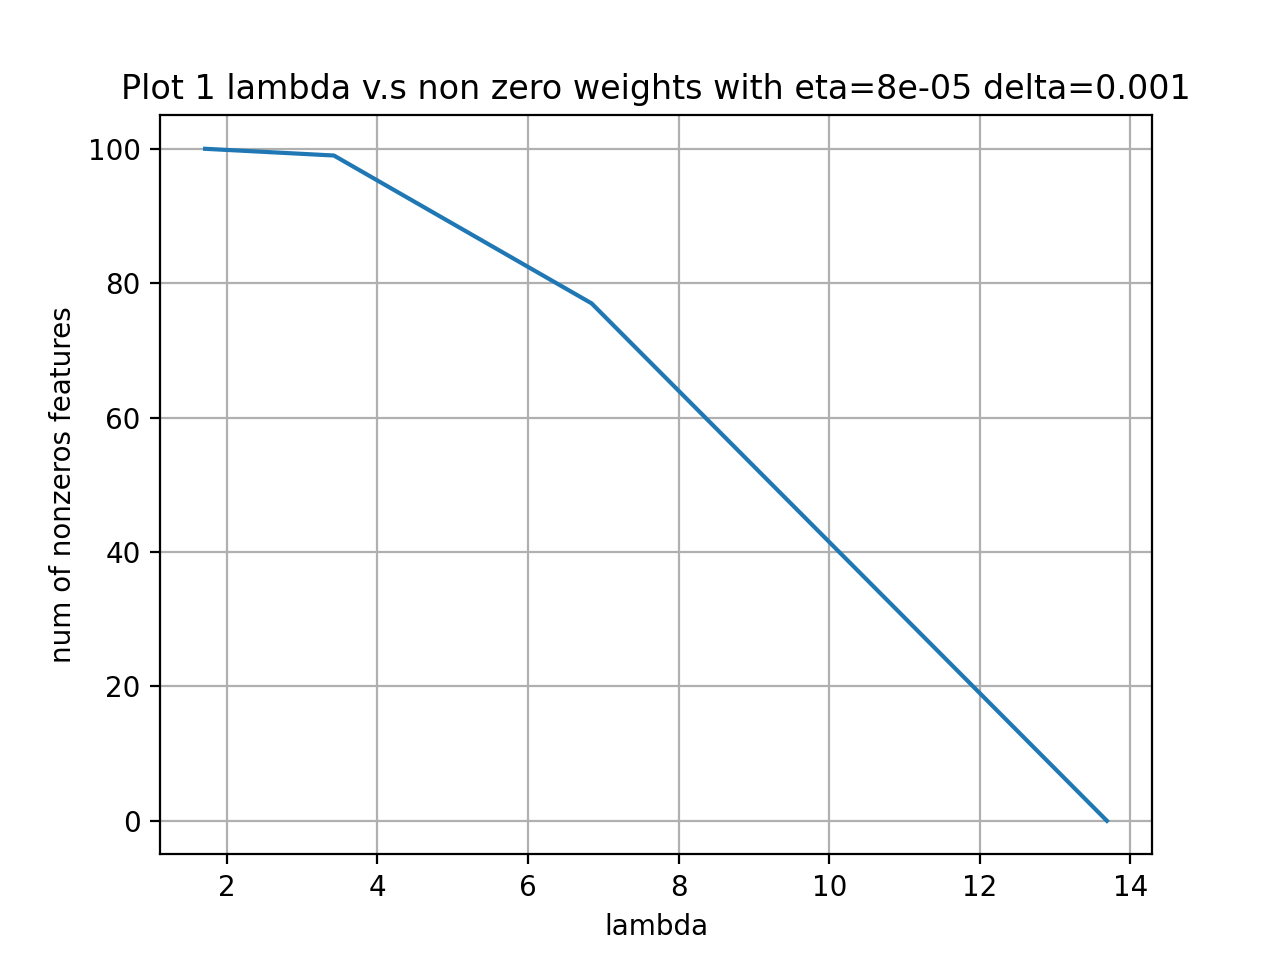
\includegraphics[width=.9\linewidth]{./img/plot1.png}
            \caption{Plot 1}
            \label{fig:plot1}
        \end{subfigure}
        \begin{subfigure}{.45\textwidth}
            \centering
            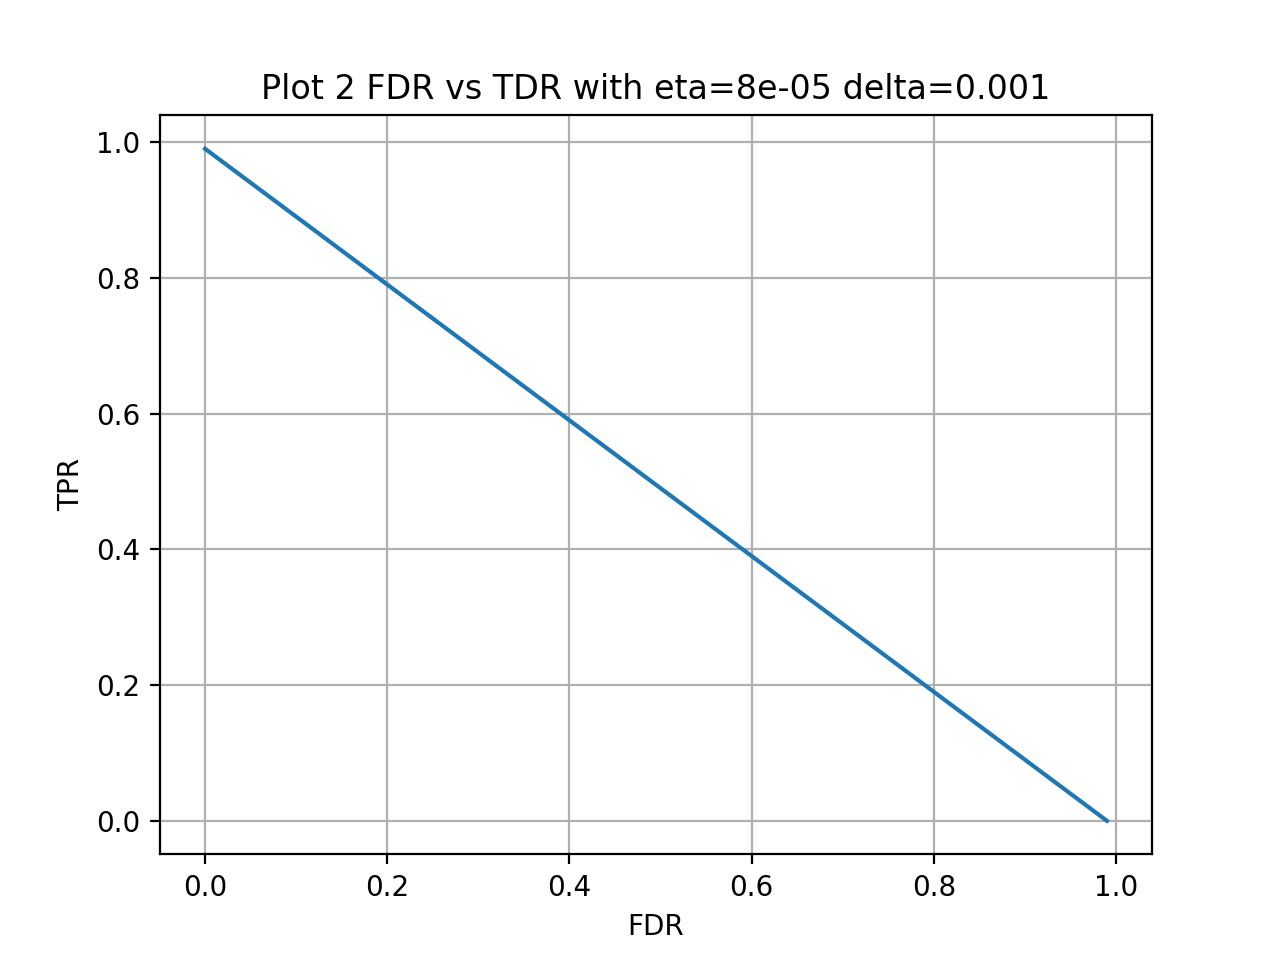
\includegraphics[width=.9\linewidth]{./img/plot2.png}
            \caption{Plot 2}
            \label{fig:plot2}
        \end{subfigure}
        \caption{A5}
    \end{figure}
    \begin{enumerate}
        \item As $\lambda$ increases, the penalty for non-zero coefficients becomes more severe, 
        pushing more coefficients to become zero, thereby reducing the number of features that contribute to the model. 
        When $\lambda$is small enough, the penalty effect is minimal and the Lasso model behaves almost like a regular linear regression, 
        typically with many non-zero coefficients.
        \item Figure \ref{fig:plot2} shows as the of number of correct nonzeros increases, 
        the incorrect nonzeros in $\widehat{w}$/total number decreasing. The two are negatively correlated.
        
    \end{enumerate}
  \end{aprob}
  
\begin{aprob}
    \label{crime} 
    We'll now put the Lasso to work on some real data in \texttt{crime\_data\_lasso.py}. We have read in the data for you with the following:
    
    \begin{verbatim}
        df_train, df_test = load_dataset("crime")
    \end{verbatim}

    This stores the data as Pandas \texttt{DataFrame} objects. \texttt{DataFrame}s are similar to Numpy \texttt{array}s but more flexible; unlike \texttt{array}s, \texttt{DataFrame}s store row and column indices along with the values of the data. Each column of a \texttt{DataFrame} can also store data of a different type (here, all data are floats). 
    Here are a few commands that will get you working with Pandas for this assignment:

    \begin{verbatim}
        df.head()                   # Print the first few lines of DataFrame df.
        df.index                    # Get the row indices for df.
        df.columns                  # Get the column indices.
        df[``foo'']                # Return the column named ``foo''.
        df.drop(``foo'', axis = 1)  # Return all columns except ``foo''.
        df.values                   # Return the values as a Numpy array.
        df[``foo''].values         # Grab column foo and convert to Numpy array.
        df.iloc[:3,:3]              # Use numerical indices (like Numpy) to get 3 rows and cols.
    \end{verbatim}

    The data consist of local crime statistics for 1,994 US
    communities. The response $y$ is the rate of violent crimes reported per capita in a community. The name of the response variable is \texttt{ViolentCrimesPerPop}, and it is held in the first column of \texttt{df\_train} and \texttt{df\_test}. There are 95 features. These
    features include many variables.
    
    Some features are the consequence of complex political processes, such as the size of the police force and other systemic and historical factors. Others are demographic
    characteristics of the community, including self-reported statistics about race, age, education, and employment drawn from Census reports.\\
    %
    The goals of this problem are threefold: ($i$) to encourage you to think about how data collection processes affect the resulting model trained from that data; ($ii$) to encourage you to think deeply about models you might train and how they might be misused; and ($iii$) to see how Lasso encourages sparsity of linear models in settings where $d$ is large relative to $n$. {\bf We emphasize that training a model on this dataset can suggest a degree of correlation between a community's demographics and the rate at which a community experiences and reports violent crime. We strongly encourage students to consider why these correlations may or may not hold more generally, whether correlations might result from a common cause, and what issues can result in misinterpreting what a model can explain.}\\
    %
    The dataset is split into a training and test set with 1,595 and 399 entries, respectively\footnote{The features have been standardized to have mean 0 and variance 1.}. 
    We will use this training set to fit a model to predict
    the crime rate in new communities and evaluate model performance on the test set.  As there are a considerable number of input variables and fairly few training observations, overfitting is a serious issue.
    In order to avoid this, use the ISTA Lasso algorithm implemented in the previous problem. 

    \begin{enumerate}
        \item \points{4} Read the documentation for the originalcversion of this dataset: \url{http://archive.ics.uci.edu/ml/datasets/communities+and+crime}. Report 3 features included in this dataset for which historical \emph{policy} choices in the US would lead to variability in these features. As an example, the \emph{number of police} in a community is often the consequence of decisions made by governing bodies, elections, and amount of tax revenue available to decision makers. Provide a short (1-3 sentence) explanation.
        \item \points{4} Before you train a model, describe 3 features in the dataset which might, if found to have nonzero weight in model, be interpreted as \emph{reasons} for higher levels of violent crime, but which might actually be a \emph{result} rather than (or in addition to being) the cause of this violence. Provide a short (1-3 sentence) explanation.
    \end{enumerate}

    Now, we will run the Lasso solver. Begin with $\lambda = \lambda_{\max}$ defined in Equation \eqref{eqn:lasso-lambdamax}. 
    Initialize all weights to $0$. Then, reduce $\lambda$ by a factor of 2 and run again, but this time initialize $\hat{{w}}$ from your $\lambda = \lambda_{\max}$ solution as your initial weights, as described above. Continue the process of reducing $\lambda$ by a factor of 2 until $\lambda < 0.01$.
    For all plots use a log-scale for the $\lambda$ dimension (Tip: use
    \verb|plt.xscale('log')|).
    \\ 
    
    
    \begin{enumerate}
        \item[c.] \points{4} Plot the number of nonzero weights of each solution as a function of $\lambda$.
        \item[d.] \points{4} Plot the regularization paths (in one plot) for the coefficients for input variables \texttt{agePct12t29}, \texttt{pctWSocSec}, \texttt{pctUrban}, \texttt{agePct65up}, and \texttt{householdsize}.
        \item[e.] \points{4} On one plot, plot the mean squared error on the training and test data as a function of $\lambda$.
        \item[f.] \points{4} Sometimes a larger value of $\lambda$ performs nearly as well as a smaller value, but a larger value will select fewer variables and perhaps be more interpretable.  Retrain and inspect the weights $\hat{w}$ for $\lambda = 30$ and for \textit{all} input variables.  Which feature had the largest (most positive) Lasso coefficient? What about the most negative? Discuss briefly.
        \item[g.] \points{4} Suppose there was a large negative weight on \texttt{agePct65up} and upon seeing this result, a politician suggests policies that encourage people over the age of 65 to move to high crime areas in an effort to reduce crime. What is the (statistical) flaw in this line of reasoning? (Hint: fire trucks
        are often seen around burning buildings, do fire trucks cause fire?)
    \end{enumerate}  

    \subsection*{What to Submit:}
    \begin{itemize}
        \item \textbf{Parts a, b:} 1-2 sentence explanation.
        \item \textbf{Part c:} Plot 1.
        \item \textbf{Part d:} Plot 2.
        \item \textbf{Part e:} Plot 3.
        \item \textbf{Parts f, g:} Answers and 1-2 sentence explanation.
        \item \textbf{Code} on Gradescope through coding submission.
        \item \textbf{All code you wrote} in the write-up, with correct page mapping.
    \end{itemize}
    \subsection{Answers}
        \begin{enumerate}
            \item \texttt{Percent of Police that are African American}: Government efforts to increase diversity in law enforcement can affect this percentage.
            \texttt{Percent of Population Who Have Immigrated within the Last 3 Years}: Immigration policies and reforms, such as the Immigration and Nationality Act amendments, impact the number and demographics of new immigrants.
            \texttt{Percentage of Males Who Have Never Married}: The benefits and disadvantages that may arise from the enactment and revision of the provisions of marriage laws, such as the cost of divorce, may affect whether people get married.
            \item \texttt{Takeotal requests for police per police officer},
            \texttt{percent of officers assigned to drug units}, and 
            \texttt{police operating budget}. These factors may be both causes and results of violence; for instance, higher violence rates may lead to more police requests and a larger portion of officers in drug units, 
            while effective use of police resources might reduce violence.
            \item 
            \begin{figure}[!h]
                \centering
                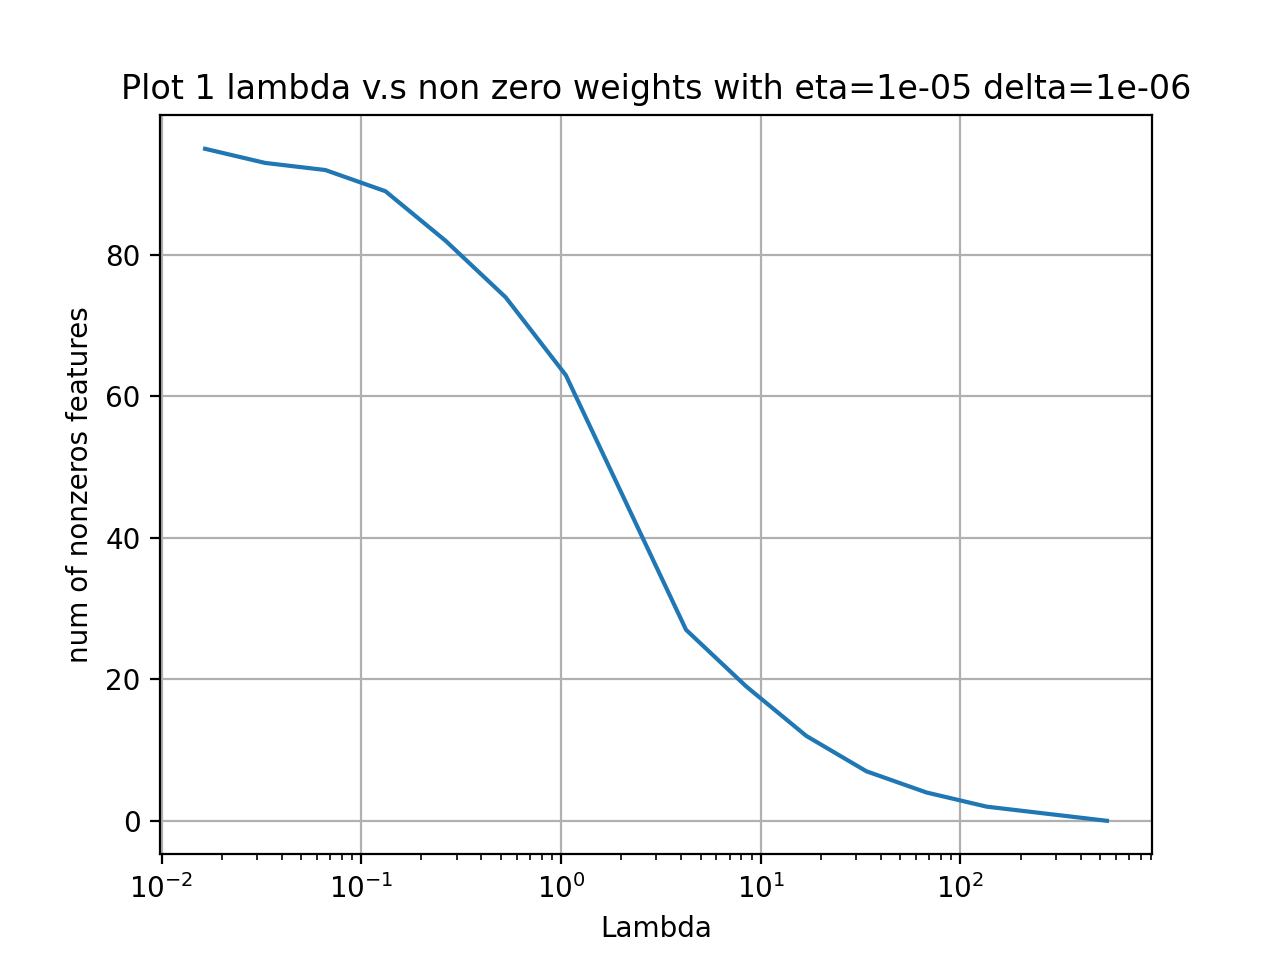
\includegraphics[width=.5\textwidth]{./img/6plot1.png}
                \caption{The number of nonzero weights of each solution as a function of $\lambda$}
                \label{fig:nonzeros}
            \end{figure}
            \item \begin{figure}[!h]
                \centering
                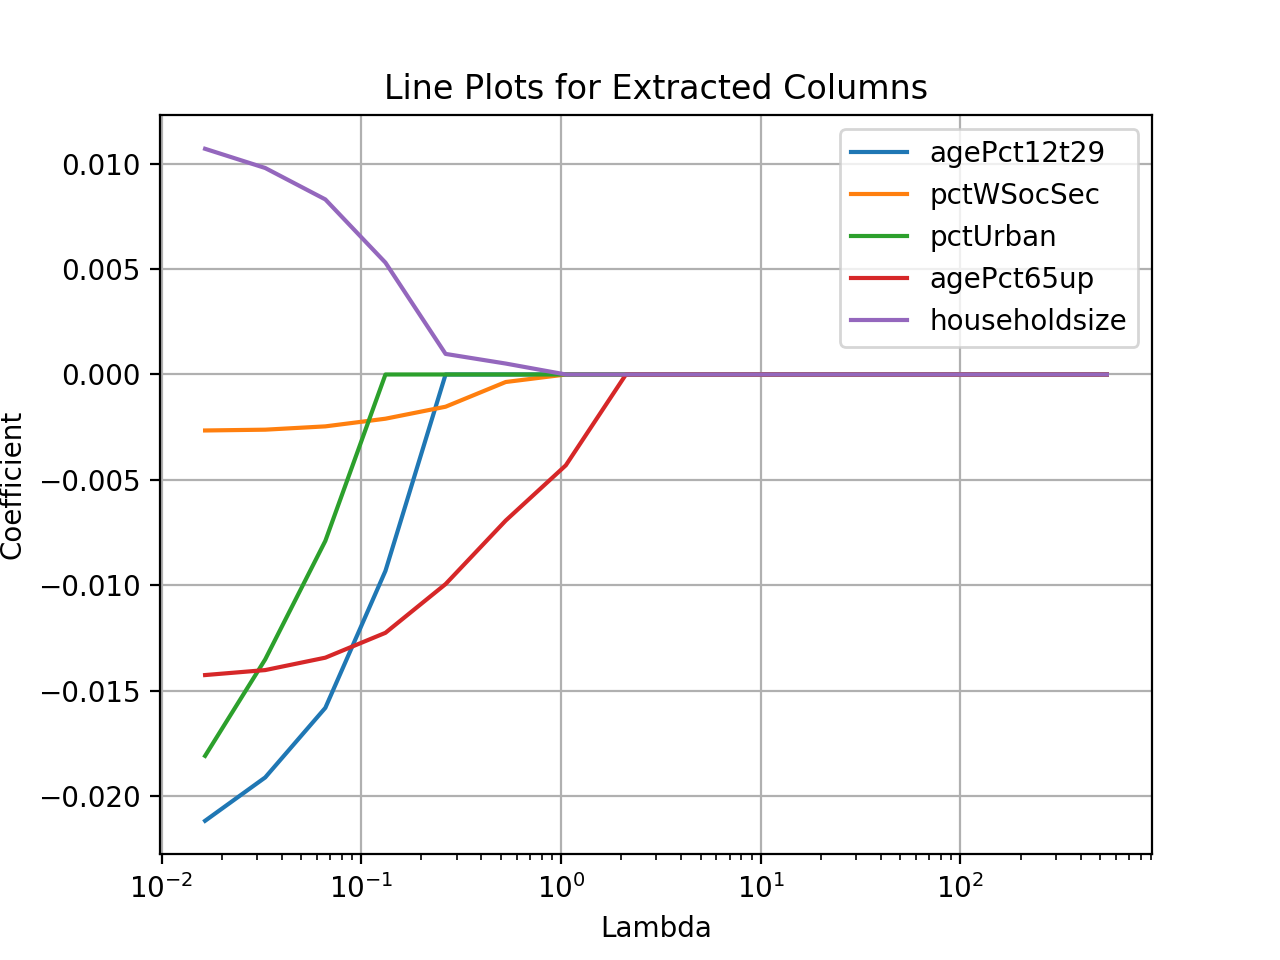
\includegraphics[width=.5\textwidth]{./img/6plot2.png}
                \caption{Plot the regularization paths}
                \label{fig:reg_paths}
            \end{figure}
            \item \begin{figure}[!h]
                \centering
                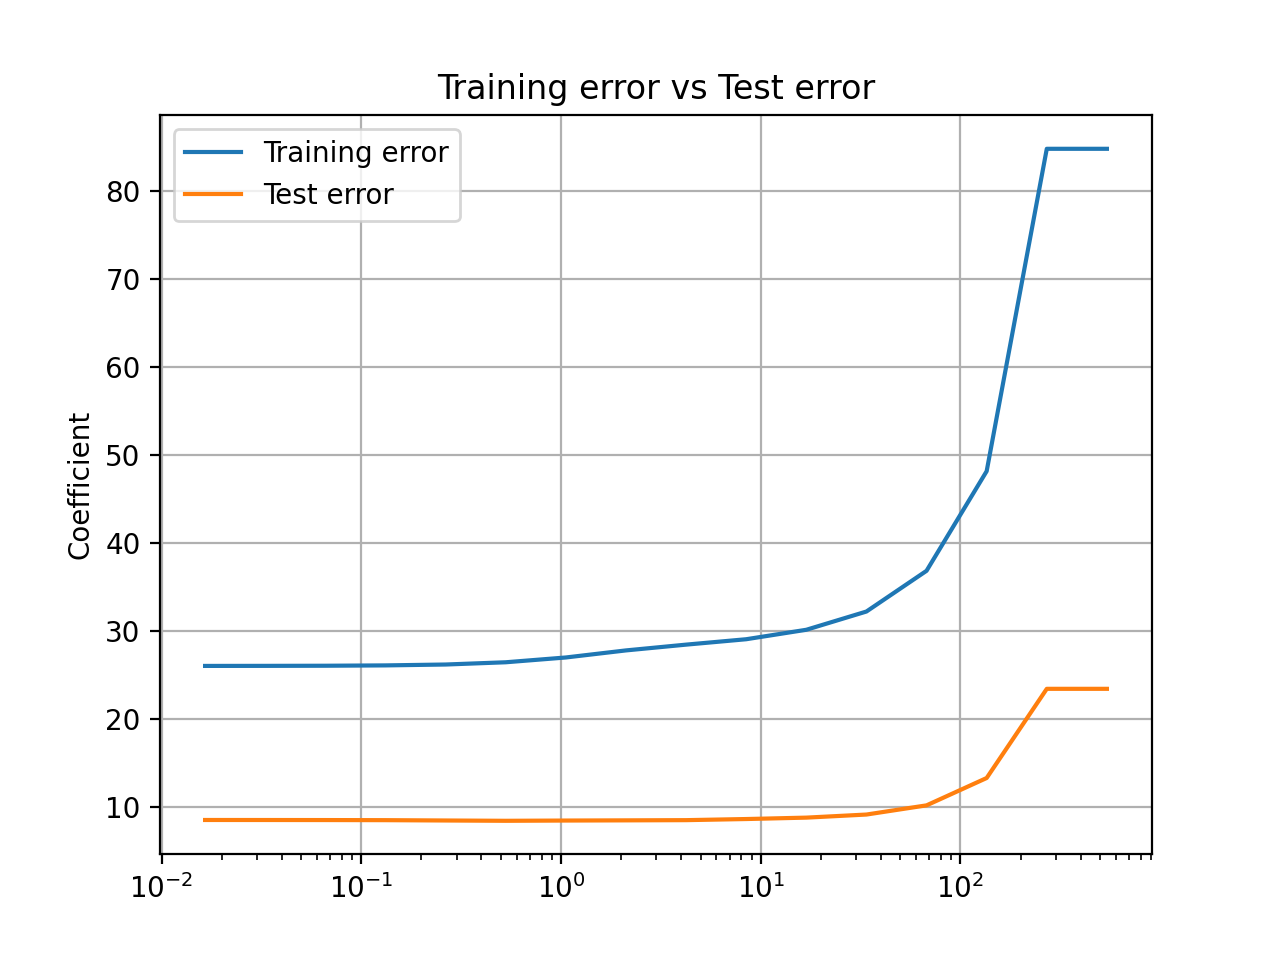
\includegraphics[width=.5\textwidth]{./img/6plot3.png}
                \caption{mean squared error on the training and test data as a function of $\lambda$}
                \label{fig:mse}
            \end{figure}
            \item \texttt{PersPerOccupHous} (mean persons per household) suggests that there is a positive correlation between the number of people living in a household and the crime rate,
            This could potentially be explained by socioeconomic factors; for example, higher household occupancy might be correlated with lower income or socioeconomic status, which in turn could be related to higher crime rates in some areas.
            However, a negative coefficient for  \texttt{PctKids2Par} (percentage of kids in family housing with two parents) indicates a negative correlation with the crime rate.
            This could be interpreted to mean that family stability or parental supervision, which is more likely in two-parent households, may be associated with lower crime rates.
            \item The negative weight on \texttt{agePct65up} in the Lasso regression model indicates that there is a correlation between higher percentages of the population being over the age of 65 and lower crime rates in the data used to train the model.
            The presence of people over 65 and the crime rate, it does not imply that one causes the other.
            It's possible that lower crime rates cause more people over 65 to move to or remain in an area, rather than the other way around.
        \end{enumerate}
\end{aprob}

% \newpage

\section*{Logistic Regression}
% \subsection*{Binary Logistic Regression} 

\begin{aprob}
    Here we consider the MNIST dataset, but for binary classification. Specifically, the task is to determine whether a digit is a $2$ or $7$.
    Here, let $Y=1$ for all the ``7'' digits in the dataset, and use $Y=-1$ for ``2''.
    We will use regularized logistic regression. 
    Given a binary classification dataset $\{(x_i,y_i)\}_{i=1}^n$ for $x_i \in \R^d$ and $y_i \in \{-1,1\}$ we showed in class that the regularized negative log likelihood objective function can be written as
    \begin{align*}
    J(w,b) = \frac{1}{n} \sum_{i=1}^n \log( 1 + \exp(-y_i (b + x_i^T w))) + \lambda ||w||_2^2
    \end{align*} 

    Note that the offset term $b$ is not regularized. 
    For all experiments, use $\lambda = 10^{-1}$. 
    Let $\mu_i(w,b) = \frac{1}{1+ \exp(-y_i (b + x_i^T w))}$. 
    \begin{enumerate}
        \item \points{8} Derive the gradients $\nabla_w J(w,b)$, $\nabla_{b} J(w,b)$ and give your answers in terms of $\mu_i(w,b)$ (your answers should not contain exponentials).
        \item \points{8} Implement gradient descent with an initial iterate of all zeros. Try several values of step sizes to find one that appears to make convergence on the training set as fast as possible. Run until you feel you are near to convergence.
        \begin{enumerate}[(i)]
            \item For both the training set and the test, plot $J(w,b)$ as a function of the iteration number (and show both curves on the same plot).  
            \item For both the training set and the test, classify the points according to the rule $\text{sign}(b + x_i^T w)$ and plot the misclassification error as a function of the iteration number (and show both curves on the same plot). 
        \end{enumerate}
          
        Reminder: Make sure you are only using the test set for evaluation (not for training).
          
        \item \points{7} Repeat (b) using stochastic gradient descent with a batch size of 1. Note, the expected gradient with respect to the random selection should be equal to the gradient found in part (a). Show both plots described in (b) when using batch size 1. Take careful note of how to scale the regularizer.
        \item \points{7} Repeat (b) using mini-batch gradient descent with batch size of 100. That is, instead of approximating the gradient with a single example, use 100. Note, the expected gradient with respect to the random selection should be equal to the gradient found in part (a).
    \end{enumerate}
    
    \subsection*{What to Submit}
    \begin{itemize}
        \item \textbf{Part a:} Proof
        \item \textbf{Part b:} Separate plots for b(i) and b(ii).
        \item \textbf{Part c:} Separate plots for c which reproduce those from b(i) and b(ii) for this case.
        \item \textbf{Part d:} Separate plots for c which reproduce those from b(i) and b(ii) for this case.
        \item \textbf{Code} on Gradescope through coding submission.
        \item \textbf{All code you wrote in the write-up, with correct page mapping.}
    \end{itemize}
    \subsection{Answers}
    \begin{enumerate}
        \item 
            %respect to w
            \begin{align*}
                J(w,b) &= \frac{1}{n} \sum_{i=1}^n \log( 1 + \exp(-y_i (b + x_i^T w))) + \lambda ||w||_2^2 \\
                % J(w,b) &= \frac{1}{n} \sum_{i=1}^n \log( 1/(\mu_i(w, b))) + \lambda ||w||_2^2 \\
                % J(w,b) &= \frac{1}{n} \sum_{i=1}^n -\log(\mu_i(w, b)) + \lambda ||w||_2^2 \\
                \nabla_w J(w,b) &= \nabla_w \Big (\frac{1}{n} \sum_{i=1}^n \log(\exp(-y_i (b + x_i^T w))) + \lambda ||w||_2^2 \Big)\\
                &= \frac{1}{n} \sum_{i=1}^n \frac{\nabla_w \exp(-y_i (b + x_i^T w))}{1 + \exp(-y_i (b + x_i^T w))} + 2 \lambda w\\
                &= \frac{1}{n} \sum_{i=1}^n \frac{\exp(-y_i (b + x_i^T w))}{1 + \exp(-y_i (b + x_i^T w))} \nabla_w(-y_i (b + x_i^T w)) + 2 \lambda w \\
                &= \frac{1}{n} \sum_{i=1}^n \frac{\exp(-y_i (b + x_i^T w))}{1 + \exp(-y_i (b + x_i^T w))} (-y_i x_i) + 2 \lambda w \\
                &= \frac{1}{n} \sum_{i=1}^n \frac{1+\exp(-y_i (b + x_i^T w)) -1}{1 + \exp(-y_i (b + x_i^T w))} (-y_i x_i) + 2 \lambda w \\
                &= \frac{1}{n} \sum_{i=1}^n (1 - \frac{1}{1 + \exp(-y_i (b + x_i^T w))} )(-y_i x_i) + 2\lambda w \\
                \nabla_w J(w,b) &= \frac{1}{n} \sum_{i=1}^n (1 - \mu_i(w, b)) (-y_i x_i) + 2\lambda w \\
            \end{align*} 
            % respect to b
            \begin{align*}
                \nabla_b J(w,b) &= \nabla_b \Big (\frac{1}{n} \sum_{i=1}^n \log( 1 + \exp(-y_i (b + x_i^T w))) + \lambda ||w||_2^2 \Big)\\
                &= \frac{1}{n} \sum_{i=1}^n \frac{\nabla_b \exp(-y_i (b + x_i^T w))}{1 + \exp(-y_i (b + x_i^T w))} + 0\\
                &= \frac{1}{n} \sum_{i=1}^n \frac{\exp(-y_i (b + x_i^T w))}{1 + \exp(-y_i (b + x_i^T w))} \nabla_b(-y_i (b + x_i^T w)) \\
                &= \frac{1}{n} \sum_{i=1}^n \frac{\exp(-y_i (b + x_i^T w))}{1 + \exp(-y_i (b + x_i^T w))} (-y_i) \\
                \nabla_b J(w,b) &= \frac{1}{n} \sum_{i=1}^n (1-\mu_i(w, b)) (-y_i)
                \end{align*}
            \begin{figure}
                \centering
                \begin{subfigure}{0.45\textwidth}
                    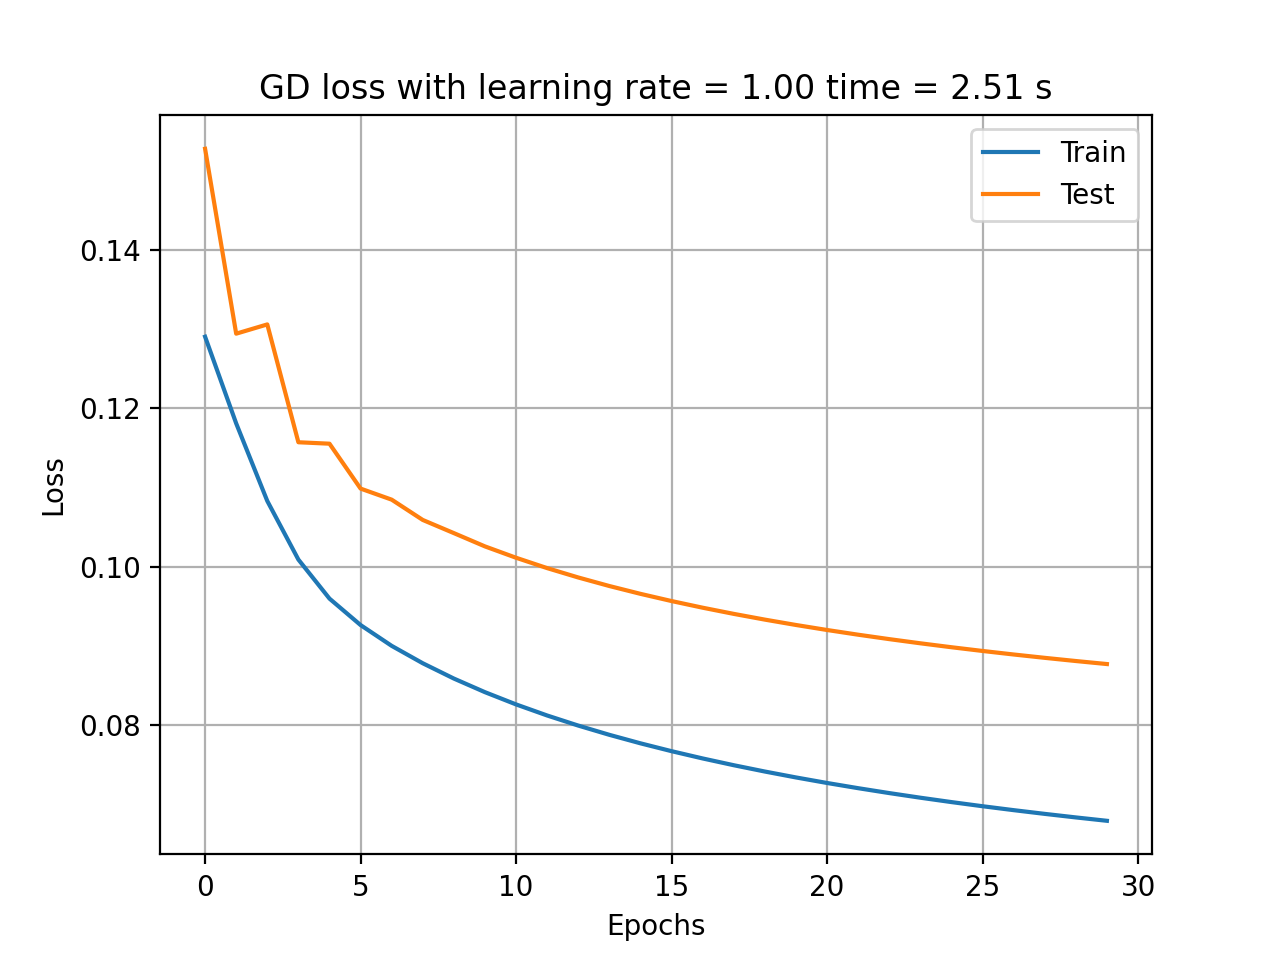
\includegraphics[width=\textwidth]{./img/7-gd-loss.png}
                    \caption{GD loss}
                    \label{fig:gdloss}
                \end{subfigure}
                \hfill
                \begin{subfigure}{0.45\textwidth}
                    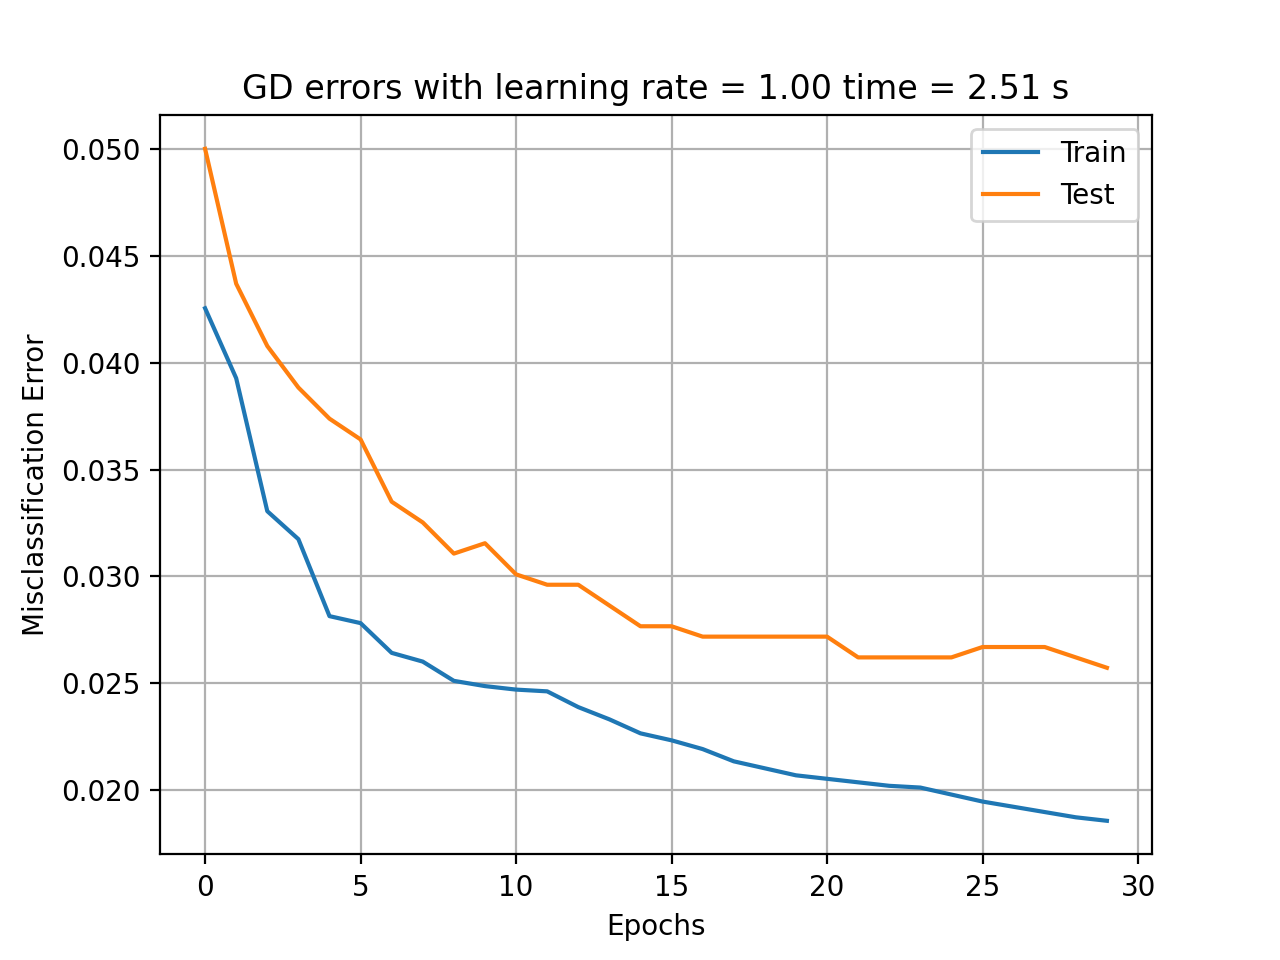
\includegraphics[width=\textwidth]{./img/7-gd-errors.png}
                    \caption{GD errors}
                    \label{fig:gderrors}
                \end{subfigure}
                \hfill
                \begin{subfigure}{0.45\textwidth}
                    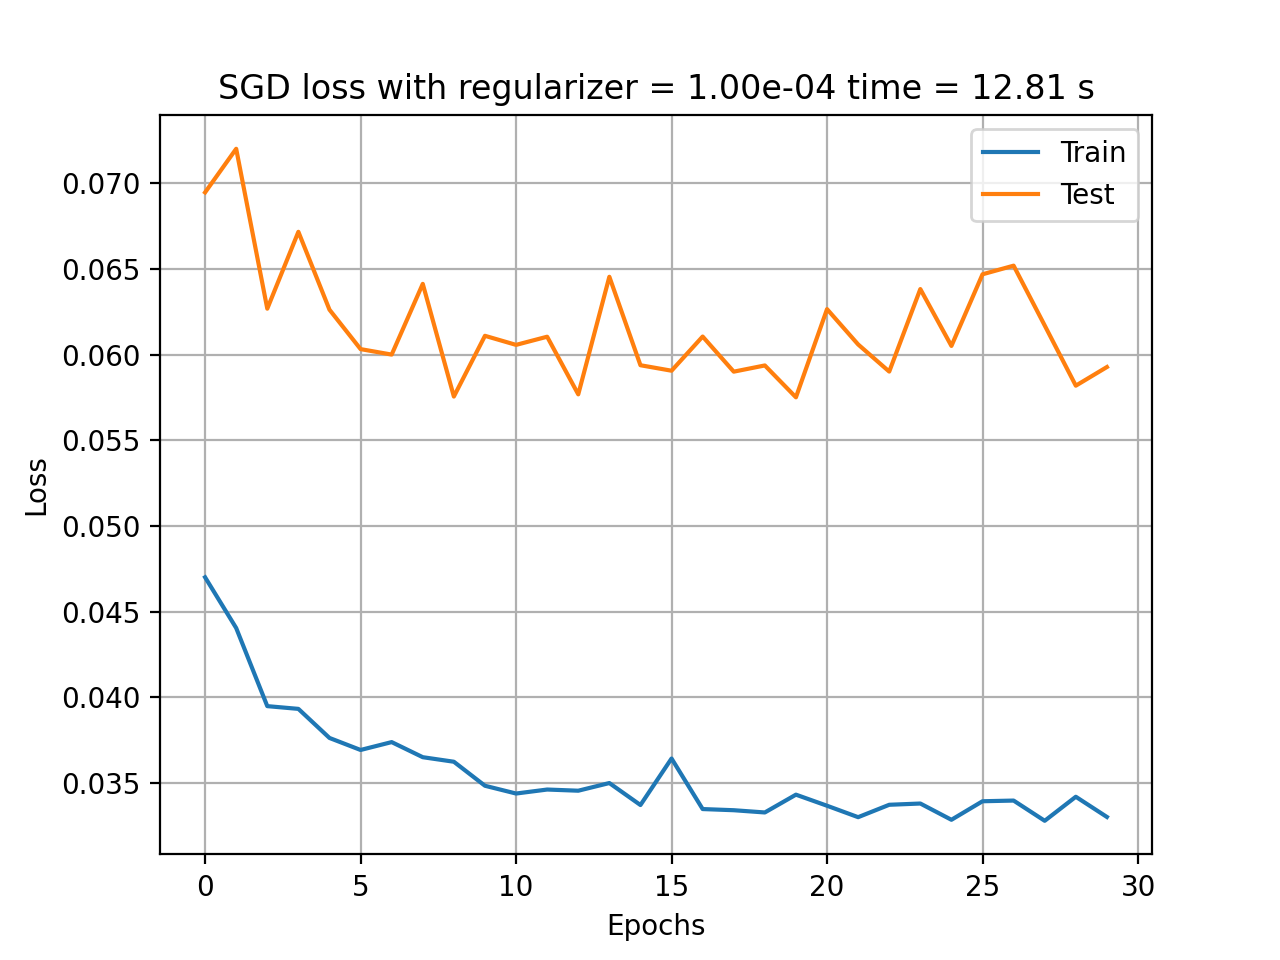
\includegraphics[width=\textwidth]{./img/7-sgd-loss.png}
                    \caption{SGD loss}
                    \label{fig:sgdloss}
                \end{subfigure}
                \hfill
                \begin{subfigure}{0.45\textwidth}
                    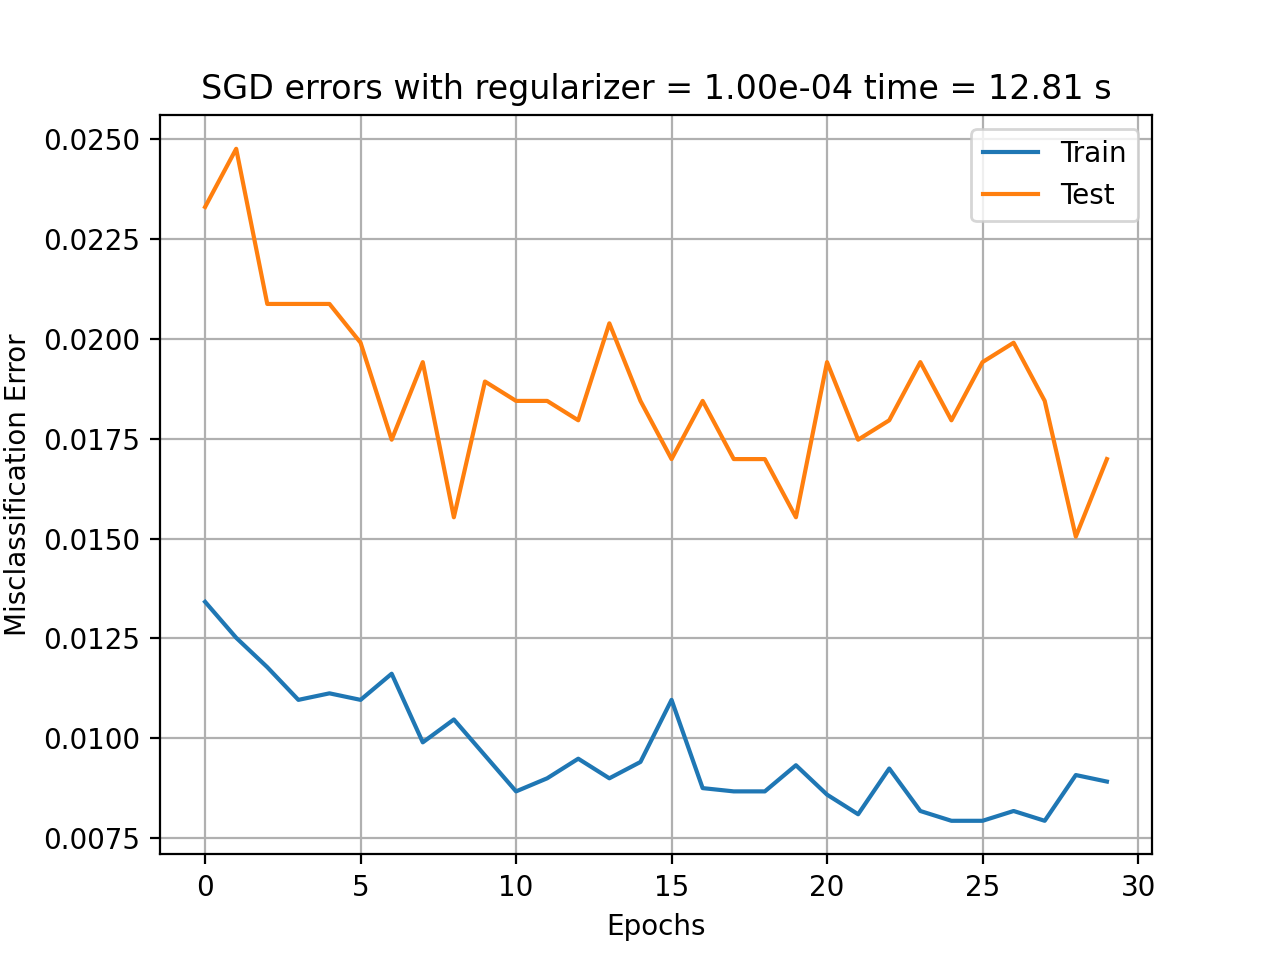
\includegraphics[width=\textwidth]{./img/7-sgd-errors.png}
                    \caption{SGD errors}
                    \label{fig:sgderrors}
                \end{subfigure}
                \begin{subfigure}{0.45\textwidth}
                    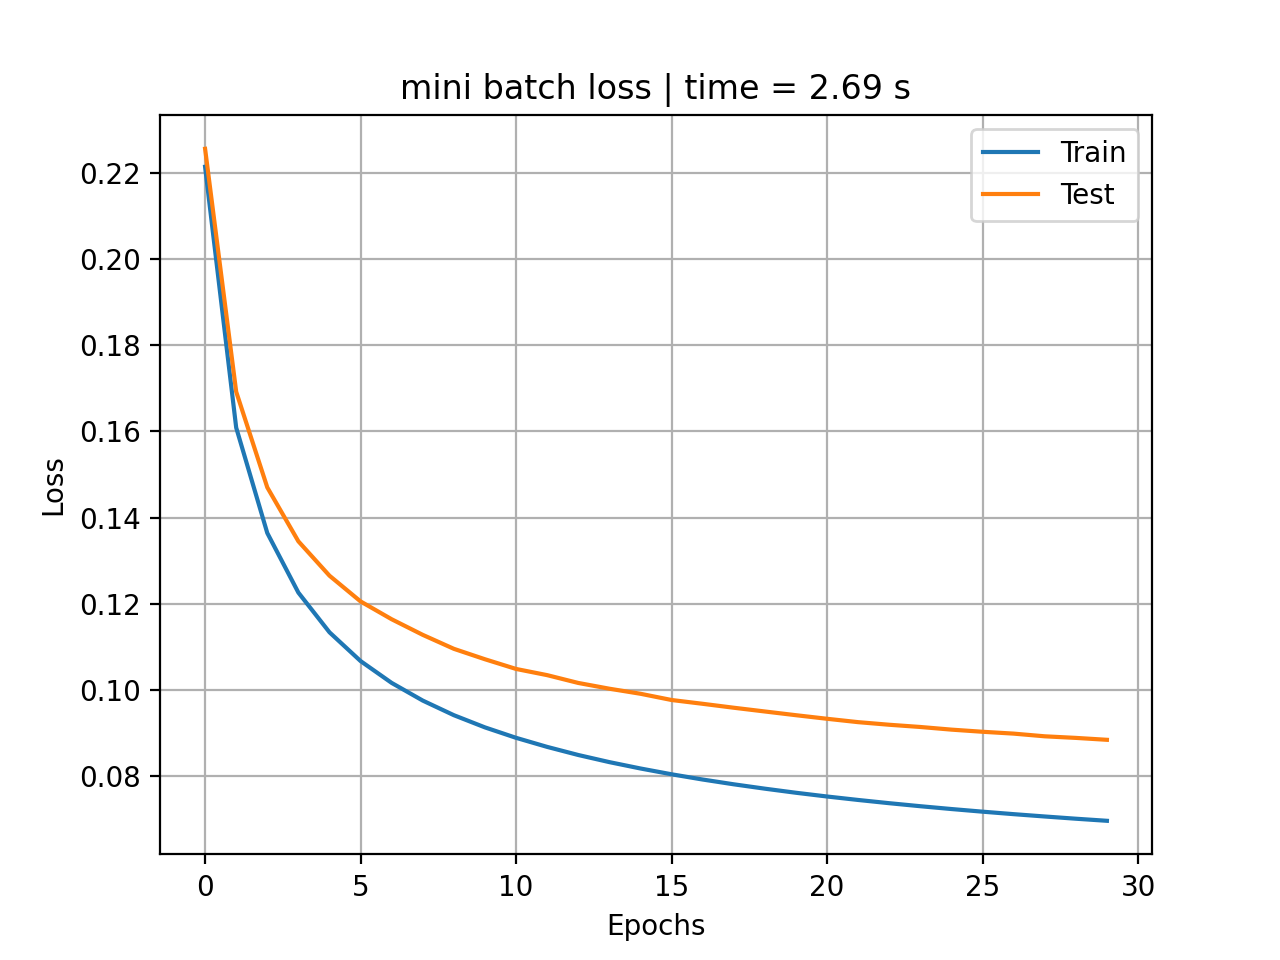
\includegraphics[width=\textwidth]{./img/7-mini-loss.png}
                    \caption{mini-batch loss}
                    \label{fig:miniloss}
                \end{subfigure}
                \hfill
                \begin{subfigure}{0.45\textwidth}
                    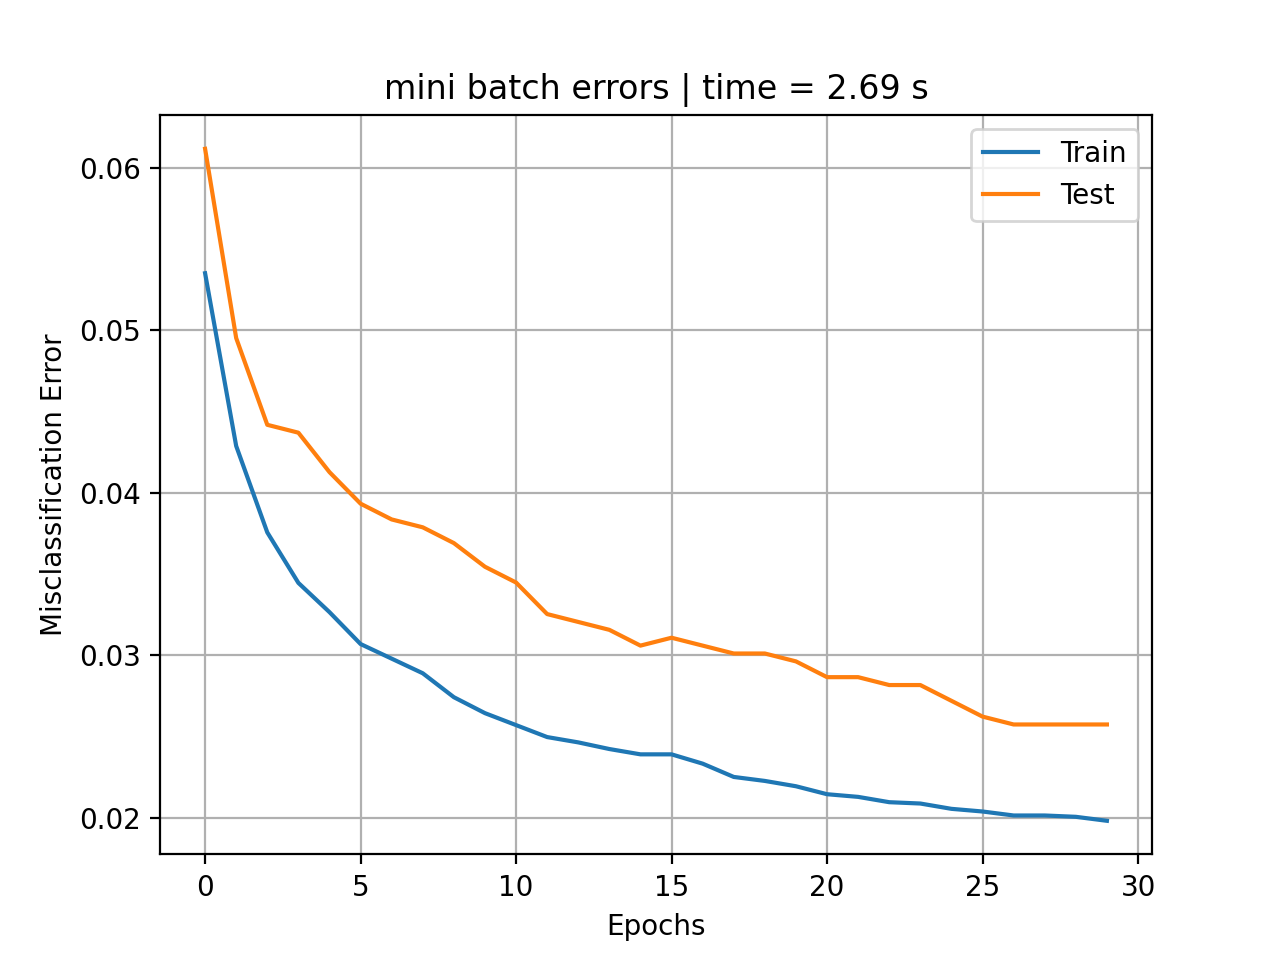
\includegraphics[width=\textwidth]{./img/7-mini-errors.png}
                    \caption{mini-batch errors}
                    \label{fig:minierrors}
                \end{subfigure}                        
                \caption{A7}
                \label{fig:a7}
            \end{figure}
    \end{enumerate}
\end{aprob}

% \newpage

\section*{Administrative}
\begin{aprob}
\begin{enumerate}
    \item \points{2} About how many hours did you spend on this homework? There is no right or wrong answer :) \\
    About 40 hours
\end{enumerate}
\end{aprob}
\end{sloppypar}
\end{document}